\documentclass[ASNA,twocolumn]{USG}
\usepackage{amsmath,amssymb,booktabs,multirow}
\usepackage{graphicx}
\usepackage{url}

\graphicspath{{./images/}}
\DeclareGraphicsExtensions{.pdf,.png,.jpg,.jpeg,.mps,.eps}
\articletype{ORIGINAL ARTICLE}%
\subarticletype{Computer Vision and Industrial Inspection}

\received{Chuangqian (author-edited draft)}
\revised{}
\accepted{}
\journal{International Journal of Imaging Systems and Technology}
\volume{0}
\copyyear{2026}
\startpage{1}
\articledoi{10.1002/0000}

\begin{document}
\title{When Does Low-Light Image Restoration Help Industrial Anomaly Detection?}
\transtitle{When Does Low-Light Image Restoration Help Industrial Anomaly Detection?}
\author[1]{Jin Huang}[https://orcid.org/0009-0005-7489-2018]
\author[2]{Qisen Gao}

\authormark{HUANG \textsc{et al.}}
\titlemark{Low-Light Restoration for Industrial Anomaly Detection}

\address[1]{\orgdiv{Faculty of Computer and Information Engineering, }\orgname{GuangXi Vocational Normal University, }\orgaddress{Nanning 530007, }\country{China}}
\address[2]{\orgname{Gansu University of Political Science and Law, }\orgaddress{Lanzhou 730070, }\country{China}}

\corres{Jin Huang (\email{614938561@qq.com})}

\fundingInfo{This research received no external funding.}

\keywords{low-light enhancement | industrial inspection | anomaly detection | image restoration | PatchCore | domain robustness}

\abstract[ABSTRACT]{Low illumination reduces both the visibility and the reliability of industrial
image inspection. We study the question of when low-light restoration actually helps downstream
industrial anomaly detection, rather than assuming that better visibility implies better inspectability.
We first introduce ICRA-MIRNet, an illumination-conditioned residual adapter wrapped around a
pretrained MIRNet-v2 backbone and fine-tuned on normal industrial training images under a
deterministic camera-inspired low-light formation model. We then fix an ImageNet-pretrained PatchCore
probe~\cite{roth2022patchcore} and evaluate clear, darkened, and restored inputs across all 15 MVTec AD
categories at mild, training-range, and severe degradation. Restoration improves training-range
anomaly AUROC from 0.800 to 0.938 ($+0.138$), but the gain shrinks to $+0.018$ under mild degradation
and $+0.019$ under severe degradation, while the generic MIRNet-v2 baseline actually degrades mild
performance ($-0.016$). A label-free restore-or-bypass gate learned only from normal detector-consistency
utility cannot reliably select when to restore: it underperforms always-restore on two of three
severities, with a mean Gate-minus-Always margin of $-0.028$. The results show that restoration benefit
is condition- and method-dependent and that normal-domain consistency utility is an inadequate proxy for
anomaly-discrimination utility. Controlled synthetic evidence cannot be extended to real night-time
factory deployments.}

\maketitle

\section{Introduction}
Industrial anomaly inspection is typically developed from well-exposed training images, whereas installed
cameras may be subject to illumination gradients, photon noise, and read noise. Image enhancement can
improve visibility, but a restoration model that alters defect evidence may increase rather than reduce
inspection risk. Consequently, restoration fidelity and downstream anomaly discrimination must be
evaluated together.

MIRNet-v2 preserves high-resolution representations while exchanging contextual information across
multiple resolutions, and it supports several restoration tasks including low-light
enhancement~\cite{zamir2023mirnetv2}. Its generic output, however, is not conditioned on the spatial
illumination pattern of a specific industrial image. We therefore wrap its output residual with a
learnable illumination-conditioned gate that retains the pretrained mapping when the gate approaches one
and permits spatially selective correction after low-memory adaptation.

Our central question is not whether restoration improves visibility, which is expected, but whether it
improves downstream anomaly detection, and under which conditions it does so. We use MVTec
AD~\cite{bergmann2019mvtecad} as the primary industrial benchmark because it provides normal training
images and normal/anomalous test images across object and texture categories. A frozen PatchCore
detector~\cite{roth2022patchcore} serves as the downstream probe and is applied verbatim to clear,
synthetically darkened, and restored images so that only the input domain changes. Low-light observations
are generated deterministically from the original clear images under three severity intervals.

The intended contributions are:
\begin{itemize}
    \item an illumination-conditioned residual formulation that adapts a pretrained MIRNet-v2 model on a
    single 8-GB GPU;
    \item a leakage-controlled protocol that trains only on normal images and jointly reports PSNR, SSIM,
    and PatchCore class-macro anomaly AUROC;
    \item a controlled three-severity analysis that identifies when restoration helps, when it is
    marginal, and when it harms;
    \item a label-free restore-or-bypass gate and an explicit audit showing that normal-domain
    detector-consistency utility is an inadequate surrogate for anomaly-discrimination utility.
\end{itemize}

\section{Related Work}
\subsection{Low-Light Image Enhancement}
The LOL dataset introduced paired low- and normal-light images for supervised
enhancement~\cite{wei2018retinex}. MIRNet-v2 subsequently provided a multiscale architecture for
restoration and enhancement with high-resolution feature preservation~\cite{zamir2023mirnetv2}. Our work
does not propose a replacement restoration backbone; it studies whether a lightweight
illumination-conditioned residual adapter can preserve industrial defect evidence under a fixed
low-light protocol, and whether that preservation translates to downstream inspectability.

\subsection{Industrial Anomaly Inspection}
MVTec AD contains normal training images and normal/anomalous test images across object and texture
categories~\cite{bergmann2019mvtecad}. Memory-bank detectors such as PatchCore achieve strong
reconstruction-free unsupervised detection by matching test patches against a coreset of training
features~\cite{roth2022patchcore}. We use image-level anomaly discrimination as the downstream probe. The
probe is deliberately frozen across clear, darkened, and restored inputs so that only the image domain
changes.

\section{Method}
\subsection{Deterministic Low-Light Formation}
Let $\mathbf{y}\in[0,1]^{3\times H\times W}$ denote a clear industrial image. A seeded degradation
operator produces
\begin{equation}
\mathbf{x}=\operatorname{clip}\left(\operatorname{Poisson}\left(255\,\mathbf{y}^{\gamma}\odot\mathbf{m}\right)/255+\boldsymbol{\epsilon},0,1\right),
\end{equation}
where $\gamma$ is sampled from a fixed interval, $\mathbf{m}$ is a smooth spatial illumination plane, and
$\boldsymbol{\epsilon}$ is zero-mean Gaussian read noise. For the training-range protocol,
$\gamma\sim\mathcal{U}(2,4)$ and the read-noise standard deviation is $\mathcal{U}(0,0.02)$. The mild
interval uses $\gamma\sim\mathcal{U}(1.2,2.0)$ and read noise $\mathcal{U}(0,0.01)$, and the severe
interval uses $\gamma\sim\mathcal{U}(4.0,5.0)$ and read noise $\mathcal{U}(0.02,0.05)$. The illumination
plane uses horizontal and vertical slopes sampled independently from $\mathcal{U}(-0.30,0.30)$ and an
offset from $\mathcal{U}(0.55,0.85)$, followed by clipping to $[0.35,1]$. Poisson noise is sampled at a
255-count scale. The degradation seed is the global seed plus the image index, so each indexed pair is
reproducible.

\subsection{Illumination-Conditioned Residual Adapter}
Let $B(\mathbf{x})$ be the pretrained MIRNet-v2 output and
\begin{equation}
\ell(\mathbf{x})=0.299\mathbf{x}_R+0.587\mathbf{x}_G+0.114\mathbf{x}_B
\end{equation}
be luminance. A two-layer convolutional network predicts a spatial gate
\begin{equation}
\mathbf{g}=\sigma\left(G(1-\ell(\mathbf{x}))\right).
\end{equation}
The final restoration is
\begin{equation}
\hat{\mathbf{y}}=\mathbf{x}+\mathbf{g}\odot\left(B(\mathbf{x})-\mathbf{x}\right).
\label{eq:adapter}
\end{equation}
The final gate layer is initialized with zero weights and bias eight, so the initial gate is close to one
and Eq.~\eqref{eq:adapter} initially approximates the pretrained backbone.

\subsection{Optimization}
The training loss is
\begin{equation}
\mathcal{L}=\lVert\hat{\mathbf{y}}-\mathbf{y}\rVert_1+\lambda_{\nabla}\lVert\nabla\hat{\mathbf{y}}-\nabla\mathbf{y}\rVert_1+\lambda_g\lVert\mathbf{g}-(1-\ell(\mathbf{y}))\rVert_1,
\end{equation}
with $\lambda_{\nabla}=0.2$ and $\lambda_g=0.05$. Training uses only the normal train split and never
touches test images or anomaly labels.

\subsection{Frozen Downstream Anomaly Probe}
For each category $c$, we use the PatchCore detector~\cite{roth2022patchcore} trained on clear normal
training images only. A Wide-ResNet-50-2 backbone extracts local patch features, a greedy coreset
subsampling constructs a compact memory bank, and the anomaly score of a test patch is the squared
nearest-neighbor distance to that memory bank. Image-level scores are pooled by the maximum over patches.
The detector is frozen after training on clear images and is applied unchanged to clear, darkened, and
restored test images. AUROC is computed within each category and macro-averaged across categories.

\section{Experiments}
\subsection{Datasets and Protocol}
The local MVTec AD copy contains 3,629 normal training images and 1,725 test images across 15
categories. The restoration model sees only the training/normal split; test images never participate in
restoration optimization or PatchCore memory-bank construction. The main model processes 12,000
micro-batches using $128\times128$ crops, batch size two, four-micro-batch gradient accumulation,
automatic mixed precision, and a fixed seed. Each indexed training image receives a deterministic crop
and degradation under the global seed. Full-resolution restoration uses overlapping $128\times128$ tiles
with 16-pixel overlap.

\subsection{Metrics}
Restoration fidelity is measured by image-pooled PSNR and SSIM~\cite{wang2004ssim}. Inspection is measured
by image-level AUROC within each category, then macro-averaged without category-size weighting for clear,
darkened, and restored inputs. Runtime is the image-pooled restoration latency and peak allocated CUDA
memory is recorded for the evaluation phase only. Main-model results are the arithmetic mean and sample
standard deviation over three seeds.

\subsection{Baselines and Ablations}
The audited matrix contains: (i) the official LOL-pretrained MIRNet-v2 without industrial adaptation;
(ii) backbone fine-tuning with a fixed gate $g=1$; (iii) ICRA-MIRNet without the gradient loss; and
(iv) the complete ICRA-MIRNet. Mild and severe degradation intervals test sensitivity outside the training
range.

\begin{figure*}[t]
\centering
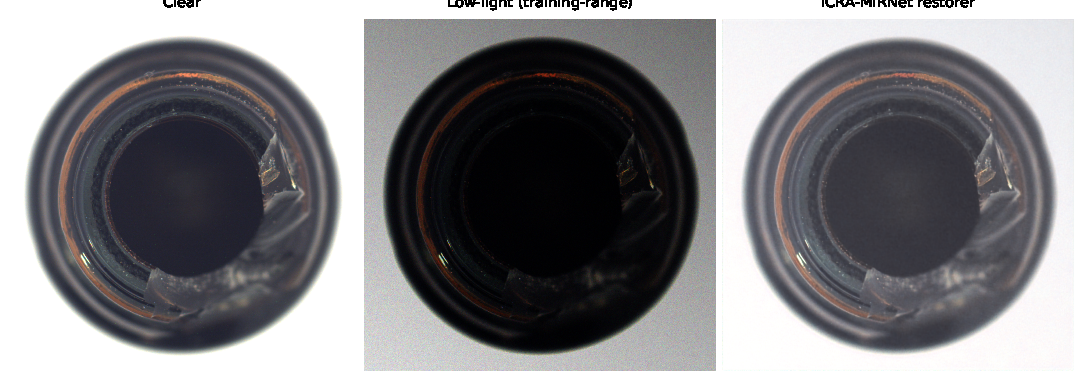
\includegraphics[width=0.94\textwidth]{fig_sample}
\caption{One MVTec AD \texttt{bottle/broken\_large} sample under training-range degradation. The clear
image (left), the deterministic low-light observation (middle), and the ICRA-MIRNet restoration (right)
share the same input content but lead to different PatchCore scores.}
\label{fig:sample}
\end{figure*}

\begin{table}[t]
\centering
\caption{MVTec AD restoration fidelity and downstream PatchCore macro AUROC for the training-range
protocol. ICRA-MIRNet reports mean $\pm$ sample standard deviation over three seeds; the LOL-pretrained
baseline and component ablations use a single seed.}
\label{tab:main}
\scriptsize
\resizebox{\columnwidth}{!}{%
\begin{tabular}{lcccc}
\toprule
Method & PSNR $\uparrow$ & SSIM $\uparrow$ & Dark AUROC & Restored AUROC\\
\midrule
LOL MIRNet-v2 & 18.168 & 0.6164 & 0.8000 & 0.8987\\
Fixed-gate fine-tuning & 28.581 & 0.8960 & 0.8000 & 0.9316\\
ICRA w/o $\mathcal{L}_{\nabla}$ & 28.744 & 0.8906 & 0.8000 & 0.9338\\
ICRA-MIRNet & $28.472\pm0.243$ & $0.8946\pm0.0015$ & $0.8000$ & $0.9378$\\
\bottomrule
\end{tabular}%
}
\end{table}

\begin{table}[t]
\centering
\caption{Class-macro PatchCore anomaly AUROC by degradation severity and input domain. Higher is better;
all rows use the frozen PatchCore detectors.}
\label{tab:severity}
\scriptsize
\resizebox{\columnwidth}{!}{%
\begin{tabular}{lcccc}
\toprule
Severity & Dark & MIRNet-v2 & ICRA-MIRNet & $\Delta$ ICRA$-$Dark\\
\midrule
mild & 0.9450 & 0.9290 & 0.9629 & $+0.0179$\\
training-range & 0.8000 & 0.8987 & 0.9378 & $+0.1378$\\
severe & 0.7569 & 0.7758 & 0.7758 & $+0.0190$\\
\bottomrule
\end{tabular}%
}
\end{table}

\begin{table}[t]
\centering
\caption{Restoration fidelity of ICRA-MIRNet across degradation severity intervals. PSNR and SSIM
are image-pooled over the restored test images. The downstream anomaly-discrimination effect is reported
separately in Table~\ref{tab:severity} using the frozen class-macro PatchCore detectors.}
\label{tab:fidelity}
\scriptsize
\resizebox{\columnwidth}{!}{%
\begin{tabular}{lcc}
\toprule
Input domain & PSNR $\uparrow$ & SSIM $\uparrow$\\
\midrule
Mild & 21.514 & 0.8640\\
Training-range & $28.472\pm0.243$ & $0.8946\pm0.0015$\\
Severe & 21.466 & 0.6521\\
\bottomrule
\end{tabular}%
}
\end{table}

\begin{figure}[t]
\centering
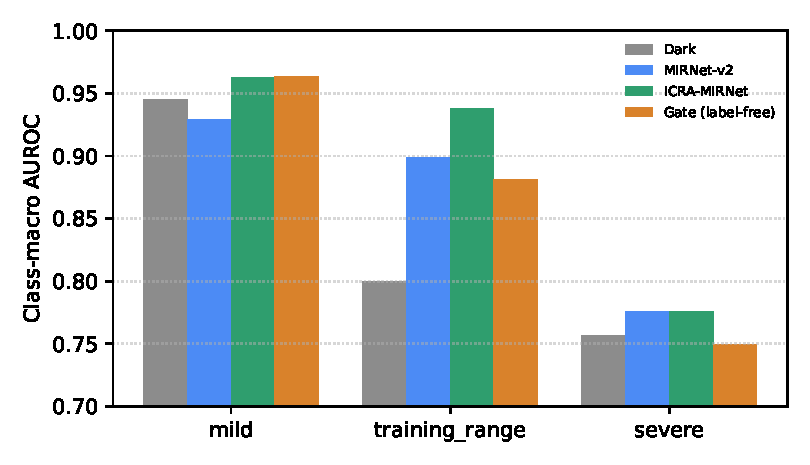
\includegraphics[width=\columnwidth]{fig_auroc}
\caption{Class-macro PatchCore AUROC by severity and input domain. Restoration helps most in
training-range, is marginal in mild/severe, and the label-free gate cannot beat always-restore on two of
three severities.}
\label{fig:auroc}
\end{figure}

\subsection{Label-Free Restore-or-Bypass Gate}
We additionally test whether a policy learned without anomaly labels can decide, per image, whether to
restore or bypass. On normal training images we define a detector-consistency utility
$U=|s_{\mathrm{dark}}-s_{\mathrm{clear}}|-|s_{\mathrm{restored}}-s_{\mathrm{clear}}|$ and label an image
as ``restore'' when $U>0$. A 23-dimensional image-only feature vector (luminance percentiles, contrast,
block statistics, gradient statistics, and a noise proxy) is fed to a standardized logistic regression.
The gate is frozen and applied image-by-image to the full test set.

The gate is not degenerate: it restores about 63\% of mild, 82\% of training-range, and 52\% of severe test
samples. However, this selectivity does not improve downstream discrimination relative to always-restore.
The repaired macro AUROC for the gate is 0.9636 (mild, $+0.0007$ vs.\ always-restore), 0.8809
(training-range, $-0.0569$), and 0.7492 (severe, $-0.0266$), with a mean Gate-minus-Always margin of
$-0.028$. Choosing to restore is not equivalent to choosing to improve anomaly detection.

\section{Reproducibility and Evidence Boundaries}
The industrial runner records configuration, checkpoints, training progress, per-image evaluation
progress, per-category metrics, and final JSON output. A separate validator rejects missing categories and
non-finite metrics before producing mean$\pm$standard-deviation tables. All low-light inputs in this study
are synthetic. Neither MVTec AD nor any available cross-dataset corpus is a paired night-time industrial
dataset, so the experiments establish controlled degradation robustness but cannot establish performance
in a real dark factory. A real paired or exposure-bracketed industrial test set remains necessary before
any deployment claim.

\section{Conclusion}
We presented an illumination-conditioned residual adapter and an audited protocol that evaluates low-light
restoration and downstream industrial anomaly discrimination together. Restoration improves training-range
PatchCore AUROC by 0.138, but the gain is only 0.018 under mild degradation and 0.019 under severe
degradation, and a generic restorer can even hurt the mild regime. A label-free gate cannot reliably
identify when restoration is useful. The mixed direction across degradation intensity, restoration method,
and policy cautions against treating restoration visibility as a proxy for inspection reliability. Future
work must add real exposure variation and an operational defect detector.

\bmsubsection*{Author Contributions}
Jin Huang conceived the study, implemented the restoration method and evaluation protocol, and wrote the
manuscript. Qisen Gao contributed to the experimental design and the analysis of downstream anomaly
detection results. Both authors approved the final manuscript. This manuscript is submitted solely to the
target journal and is not under consideration elsewhere.

\bmsubsection*{Acknowledgments}
The authors thank the anonymous reviewers for their constructive comments.

\bmsubsection*{Financial Disclosure}
This research received no external funding.

\bmsubsection*{Conflicts of Interest}
The authors declare no conflicts of interest.

\bmsubsection*{Data Availability Statement}
The derived results tables and the audited per-category records are available from the corresponding author
on reasonable request. MVTec AD is publicly available from its original authors.

\bibliography{lowlight_anomaly}

\end{document}
